% !TEX root = main.tex

\section{微积分的应用}
这一章其实最关键的是建模,即如何用微元的思想对具体问题进行刻画. 至于具体的积分计算,则是第\ref{sec:indefinite_integration}章、第\ref{sec:definite_integration}章的内容.
\subsection{面积}
\begin{enumerate}
	\item 直角坐标
	\[\diff A=y\diff x=(f(x)-g(x))\diff x\]
	\item 参数方程(简单闭曲线$\Gamma$,端点相连,其他地方不相交\footnote{规定曲线的正向:沿着曲线的正向走,其包围的有界区域始终在曲线左侧})
	\[\diff A=y(t)\diff x(t)\implies A=\textcolor{red}{-}\oint_\Gamma y\diff x\]
	\item 极坐标
	\[\diff A=\dfrac{1}{2}r^2(\theta)\diff\theta\]
\end{enumerate}

\subsection{体积}
\begin{enumerate}
	\item 旋转体
\[\diff V=\pi[f(x)]^2\diff x\]
	\item 已知截面积
\[\diff V=A(x)\diff x\]
\end{enumerate}

\subsection{弧长}
\begin{center}
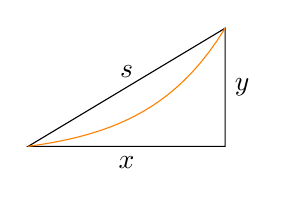
\begin{tikzpicture}[domain=0:2.5]
\draw (0,0) --node[below] {$\diff x$} (2.5,0) --node[right] {$\diff y$} (2.5,1.5) --node[left,above] {$\diff s$} cycle;
\draw[color=orange] plot (\x,{1.5/(exp(2.5)-1)*(exp(\x)-1)});
\end{tikzpicture}
\end{center}
\[\diff s=\sqrt{\diff x^2+\diff y^2}=\sqrt{1+\lrp{\dfrac{\diff y}{\diff x}}^2}\diff x\]
\begin{enumerate}
	\item 直角坐标
	\[\diff s^2=(1+[f'(x)]^2)\diff x^2\]
	\item 参数方程
	\[\diff s^2=([x(t)]^2+[y(t)]^2)\diff t^2\]
	\item 极坐标(通过$x=r\cos\theta,y=r\sin\theta$转直角坐标推导)
	\[\diff s^2=r^2\diff\theta^2+\diff r^2\]
\end{enumerate}

\subsection{曲率}
\begin{definition}[曲率]
用切线夹角与弧长之比来衡量曲线的弯曲程度,即
\[K=\left|\dfrac{\diff\varphi}{\diff s}\right|\]
\end{definition}
\begin{enumerate}
	\item 直角坐标
	\[K=\dfrac{|y''|}{(1+y'^2)^\frac{3}{2}}\]
	\item 参数方程(由参方推其他两个)
	\[K=\dfrac{|y''x'-y'x''|}{(x'^2+y'^2)^\frac{3}{2}}\]
	\item 极坐标
	\[K=\dfrac{|r^2+2r'^2-rr''|}{(r^2+r'^2)^\frac{3}{2}}\]
\end{enumerate}

\subsection{质心}
旋转体的侧面积可以通过以下的微元公式得到
\[\diff S=2\pi y\diff s\]
\begin{theorem}[古鲁金(Guldin)第一定理]
质量分布均匀的平面曲线弧的质心坐标$(\bar{x},\bar{y})$由下式得出
\[2\pi\bar{x}l=S_1\qquad 2\pi\bar{y}l=S_2\]
其中,$S_1$和$S_2$分别为曲线弧绕$y$轴和绕$x$轴所得旋转体的侧面积,$l$为弧长.
\end{theorem}
其基本思想即将旋转体的侧面积转化为圆柱的侧面积.
\begin{theorem}[古鲁金第二定理]
质量分布均匀的平面图形绕此平面上一条与之不相交的直线旋转,所得旋转体的体积由下式给出
\[V=2\pi\bar{y}S\]
\end{theorem}